\renewcommand{\theequation}{\theenumi}
\begin{enumerate}[label=\thesection.\arabic*.,ref=\thesection.\theenumi]
\numberwithin{equation}{enumi}

\item It is given that in a group of 3 students, the probability of 2 students not having the
same birthday is 0.992. What is the probability that the 2 students have the same
birthday?
\\
\solution 
We know that two students either have birthday on same date or they don't have same birthday. No other cases are possible.\\
Therefore, we can consider this as a bernoulli distribution, by defining a random variable X such that,if $X=0$, then they don't have same birthday, if $X=1$, then they have same birthday.
Therefore,
\begin{align}
Pr(X=0)+Pr(X=1)=1\\
Pr(X=0)=0.992\\
Pr(X=1)=1-Pr(X=0)\\
Pr(X=0)=1-0.992\\
Pr(X=0)=0.008
\end{align}
\item 


\item A box contains 5 red marbles, 8 white marbles and 4 green marbles. One marble is taken
out of the box at random. What is the probability that the marble taken out will be\\
(i) red ?\\
(ii) white ? \\
(iii) not green?
\\
\solution 
Total number of marbles = 5 + 8 + 4 = 17 marbles.
Let $X \in \{0,1,2\}$ represent the random variable, where 0 represents a red marble, 1 represents a white marble, and 2 represents a green marble. From the given information, 
\begin{align}
    Pr(X=0) &= \frac{5}{17} \\
    Pr(X=1) &= \frac{8}{17} \\
    Pr(X=2) &= \frac{4}{17} \implies \pr{X\ne 2} = \frac{13}{17}
\end{align}

\item A piggy bank contains hundred 50p coins, fifty rupee 1 coins, twenty rupee 2 coins and ten rupee 5 coins. If it is equally likely that one of the coins will fall out when the bank is turned upside down, what is the probability that the coin \\
(i) will be a 50 p coin ?\\
(ii) will not be a rupee5 coin?\item If each element of a second order determinant is either zero or one, what is the
probability that the value of the determinant is positive? (Assume that the individual entries of the determinant are chosen independently, each value being
assumed with probability $\frac{1}{2}$).\\
\item If a leap year is selected at random, what is the chance that it will contain 53
Tuesdays?\\
\item
\item
\item Suppose that two cards are drawn at random from a deck of cards. Let X be the number of aces obtained. Then the value of E(X) is\\
\begin{enumerate}
\item $\frac{37}{221}$
\item $\frac{5}{13}$
\item $\frac{1}{13}$
\item $\frac{2}{13}$
\end{enumerate}
\item The mean of the numbers obtained on throwing a die having written 1 on three faces, 2 on two faces and 5 on one face is\\
\begin{enumerate}
\item 1
\item 2
\item 5
\item $\frac{8}{3}$
\end{enumerate}
\item A class has 15 students whose ages are 14, 17, 15, 14, 21, 17, 19, 20, 16, 18, 20,
17, 16, 19 and 20 years. One student is selected in such a manner that each has the same chance of being chosen and the age X of the selected student is recorded. What is the probability distribution of the random variable X? Find mean, variance and standard deviation of X.\\
\solution  Table \ref{table:5.11} summarizes the given info.
\begin{table}[!ht]
\begin{center}
\begin{tabular}{|c|c|c|c|c|c|c|c|c|}
\hline
{X} & 0 & 1 & 2 & 3 & 4 & 5 & 6 & 7 \\
\hline
{No. of students} & 2 & 1 & 2 & 3 & 1 & 2 & 3 & 1 \\
\hline
{P(X)} & $\frac {2}{15}$ & $\frac {1}{15}$ & $\frac {2}{15}$ & $\frac {3}{15}$ & $\frac {1}{15}$ & $\frac {2}{15}$ & $\frac {3}{15}$ & $\frac {1}{15}$
\\
\hline 
\end{tabular}
\end{center}
\caption{}
\label{table:5.11}
\end{table}
using which, 
 \begin{align}
      E(X) &= \sum_{i=1}^n x_i \pr{X=i} = \frac{263}{15}
      \\
    E(X^2) = \sum_{i=1}^n x_i^2 \pr{X=i} =    \frac{4683}{15}
    \\
    \implies Var (X) = \frac{4683}{15} - (\frac{263}{15})^2
    = 4.78
    \end{align}
\item A random variable X has the following probability distribution:\\
\\$\begin{tabular}{||c c c c c c c c c||} 
 \hline
 X & 0 & 1 & 2 & 3 & 4 & 5 & 6 & 7 \\
 \hline
 P(X) & 0 & k & 2k & 2k & 3k & $k^2$ & 2$k^2$ & 7$k^2$+k \\
 \hline
\end{tabular}$\\
\\Determine\\
(i) k \\
(ii) P(X < 3)\\
(iii) P(X > 6)\\
(iv) P(0 < X < 3)\\\item Find the probability distribution of the number of successes in two tosses of a die, where a success is defined as\\
(i) number greater than 4\\
(ii) six appears on at least one die\\
\item An urn contains 5 red and 2 black balls. Two balls are randomly drawn. Let X represent the number of black balls. What are the possible values of X? Is X a random variable ?\\
\item State which of the following are not the probability distributions of a random variable. Give reasons for your answer.\\
(i) \\$\begin{tabular}{||c c c c||} 
 \hline
 X & 0 & 1 & 2 \\
 \hline
 P(X) & 0.4 & 0.4 & 0.2 \\
 \hline
\end{tabular}$\\

(ii) \\$\begin{tabular}{||c c c c c c||} 
 \hline
 X & 0 & 1 & 2 & 3 & 4 \\
 \hline
 P(X) & 0.1 & 0.5 & 0.2 & -0.1 & 0.3 \\
 \hline
\end{tabular}$\\

(iii) \\$\begin{tabular}{||c c c c||} 
 \hline
 X & -1 & 0 & 1 \\
 \hline
 P(X) & 0.6 & 0.1 & 0.2 \\
 \hline
\end{tabular}$\\

(iv) \\$\begin{tabular}{||c c c c c c||} 
 \hline
 X & 3 & 2 & 1 & 0 & -1 \\
 \hline
 P(X) & 0.3 & 0.2 & 0.4 & 0.1 & 0.05 \\
 \hline
\end{tabular}$\\
\solution Only (i) is valid.  The remaining do not satisfy one of the following 
conditions.
\begin{align}
0 \le \pr{X = i} \le 1
\\
\sum_{i}\pr{X=i} = 1
\end{align}
\item A card from a pack of 52 cards is lost. From the remaining cards of the pack, two cards are drawn and are found to be both diamonds. Find the probability of the lost card being a diamond.\\
\item Suppose a girl throws a die. If she gets a 5 or 6, she tosses a coin three times and notes the number of heads. If she gets 1, 2, 3 or 4, she tosses a coin once and notes whether a head or tail is obtained. If she obtained exactly one head, what is the probability that she threw 1, 2, 3 or 4 with the die?\\
\solution 
Let $X\in\{0,1\}$ where X=0 represents that we get 1,2,3 or 4 when a die is rolled and X=1 represents that we get 5 or 6 when a die is rolled. \\
Let $Y\in\{0,1,2,3\}$ where Y=1 represents that we get exactly one head.Here Y represents the number of heads obtained. \\ 

We are required to find probability of getting X=0 when Y=1.\\
Here we use Bayes' theorem.

\begin{equation}
   \pr{X=0|Y=1}= \frac{\pr{X=0} \hspace{0.2cm} \pr{Y=1|X=0}}{\sum\limits_{i=0}^{1} \pr{X=i} \hspace{0.2cm} \pr{Y=1|X=i}}
\end{equation} 

Note that 
\begin{align}
    \pr{X=0} = \frac{4}{6} = \frac{2}{3} = 0.6666666667 \\
    \pr{X=1} = \frac{2}{6} = \frac{1}{3} = 0.3333333333
\end{align} 

Also we get
\begin{align}
    \pr{Y=1|X=0} = \frac{1}{2} = 0.5 \\
    \pr{Y=1|X=1} = \frac{3}{8} = 0.375
\end{align} 

Substituting values, we get
\begin{align}
    \pr{X=0|Y=1} = \frac{\frac{2}{3} \times \frac{1}{2}}{{\frac{2}{3} \times \frac{1}{2}} + \frac{1}{3} \times \frac{3}{8}} \\
\implies \pr{X=0|Y=1} = \frac{8}{11} = 0.7272727273
\end{align} 

\item An insurance company insured 2000 scooter drivers, 4000 car drivers and 6000 truck drivers. The probability of an accidents are 0.01, 0.03 and 0.15 respectively. One of the insured persons meets with an accident. What is the probability that he is a scooter driver?\\
\solution 
By definition
\begin{align}
\pr{A|B} = \frac{\pr{AB}}{\pr{B}} \label{5.18:1}
\end{align}
Also, by Bayes' Theorem
\begin{align}
\pr{A} = \sum_{i=1}^n \pr{A|E_i}\pr{E_i}\label{5.18:2}
\end{align}
where $E_1 , E_2 \ldots E_n$  are partitions of the complete sample set.\\

Let X be a random variable taking the following values in Table \ref{table:5.18}.
\begin{table}[!ht]
\begin{center}
\begin{tabular}{ |c|c| } 
 \hline
 X = 0 & Scooter Drivers\\
 \hline
 X = 1 & Car Drivers\\
 \hline
X = 2 & Truck Drivers\\
 \hline
\end{tabular}
\end{center}
\caption{}
\label{table:5.18}
\end{table}
where X $\in \{0, 1, 2\}$ represent all the partitions of the sample set.


Let Y be a random variable taking the following values in Table \ref{table:5.18_1}.
\begin{table}[!ht]
\begin{center}
\begin{tabular}{ |c|c| } 
 \hline
 Y = 0 & Involved in an accident\\
 \hline
 Y = 1 & Not involved in an accident\\
 \hline
\end{tabular}
\end{center}
\caption{}
\label{table:5.18_1}
\end{table}

 Also, the following values are known:
\begin{align}
\pr{X = 0} = \frac{2000}{2000+4000+6000} = \frac{1}{6}\\
\pr{X = 1} = \frac{4000}{2000+4000+6000} = \frac{1}{3}\\
\pr{X = 2} = \frac{6000}{2000+4000+6000} = \frac{1}{2}\\
\pr{Y = 0|X = 0} = 0.01\\
\pr{Y = 0|X = 1} = 0.03\\
\pr{Y = 0|X = 2} = 0.15
\end{align}

We have to find:
\begin{align}
\pr{X = 0|Y = 0} = \frac{\pr{X = 0 \cap Y = 0}}{\pr{Y = 0}}
\end{align}
Using \eqref{1} and \eqref{2}, we get:
\begin{multline}
\pr{X = 0|Y = 0} 
\\
= \frac{\pr{Y = 0|X = 0}\pr{X = 0}}{\sum_{i=0}^{i=2}\pr{Y = 0 | X = i}\pr{X = i}}
\\
= \frac{\frac{0.01}{6}}{\frac{0.01}{6} + \frac{0.03}{3} + \frac{0.15}{2}}
 = \frac{1}{52}
\end{multline}

\item A carton consists of 100 shirts of which 88 are good, 8 have minor defects and 4 have major defects.Jimmy, a trader, will only accept the shirts which are good, but Sujatha, another trader, will only reject the shirts which have major defects.One shirt is drawn at random from the carton. What is the probability that\\
(i) it is acceptable to Jimmy?\\
(ii) it is acceptable to Sujatha?
\\
\solution
Let random variable  $X\in\{0,1,2\}$ denote the outcomes of experiment of drawing a shirt from the carton as shown in Table \ref{table:}
\begin{table}[h]
\centering 
\caption{}
\begin{tabular}{|c|c|c|c|}
\hline
Type of shirt & X & number      & \pr{X}      \\
\hline
good          & 0 & n(X=0) = 88 & $\frac{22}{25}$ \\
\hline
minor defect  & 1 & n(X=1) = 8  & $\frac{2}{25}$ \\
\hline
major defect  & 2 & n(X=2) = 4  & $\frac{1}{25}$\\
\hline
\end{tabular}
\label{table:}
\end{table}

\begin{enumerate}[label={\roman*)}]
    \item The required probability is
    \begin{align}
      p &= \pr{X=0}\\
        &= \frac{88}{100}\\
        &= 0.88
    \end{align}
    \item The required probability is
    \begin{align}
        p &= \pr{X=0}+\pr{X=1}\\
          &= \frac{88}{100}+\frac{8}{100}\\
          &=0.96
    \end{align}
\end{enumerate}
\item Two dice, one blue and one grey, are thrown at the same time. Write down all the possible outcomes.What is the probability that the sum of the two numbers appearing on the top of the dice is\\
(i) 8?\\
(ii) 13?\\ 
(iii) less than or equal to 12?\\\\
\item Savita and Hamida are friends. What is the probability that both will have \\
(i) different birthdays? \\
(ii) the same birthday? (ignoring a leap year).
\item 
\item  A box contains 3 blue, 2 white, and 4 red marbles. If a marble is drawn
at random from the box, what is the probability that it will be
(i) white? (ii) blue? (iii) red?
\\
\solution 
Consider the random variable X = \{0,1,2\} represent the marble colour blue or white or red.\\
\begin{table}[ht]
\begin{tabular}{|c|c|c|c|}
\hline
\textbf{Color}&\textbf{X}&\textbf{N(X)}&\textbf{Pr(X)}  \\ \hline    
Blue  &0  &3  &3/9  \\ \hline
White  &1  &2  &2/9  \\ \hline
Red  &2  &4  &4/9  \\ \hline
\end{tabular}
\caption{Table for probabilities of marbles}
\label{table:data}
\end{table}
Picking up any marble from the box is equally - likely.
The box contain a total of 9 marbles.

\begin{align}
 \pr{X=0} = \frac{N(X=0)}{9} = \frac{3}{9}\\
 \pr{X=1} = \frac{N(X=1)}{9} = \frac{2}{9}\\
 \pr{X=2} = \frac{N(X=2)}{9} = \frac{4}{9}
\end{align}

\item One card is drawn from a well-shuffled deck of 52 cards. Calculate the
probability that the card will\\
(i) be an ace,\\
(ii) not be an ace.
\\
\solution 
For convinience, let's denote the cards Ace, J, Q, K by the numbers $\{ 1, 11, 12, 13\}$ respectively. Let $X \in \{ 1, 2, 3, 4, 5, 6, 7, 8, 9, 10, 11, 12, 13 \}$ denote the outcome of the experiment. We know that there exist exactly 4 cards with a particular number in a deck of 52 cards. Assuming that the deck of cards is well-shuffled, the probability mass function for this experiment is expressed as\\
\begin{align}
	\Pr(X=i) = 
	\begin{cases}
	\dfrac{4}{52} = \dfrac{1}{13} & 1 \leq i \leq 13, \; i \in \mathbb{N}\\ ~\\[-1em]
	0 & \text{otherwise}
	\end{cases}
\end{align}
\begin{enumerate}[label = (\roman*)]
\item Hence, the probability of getting an Ace is 
\begin{align}
	\Pr(X=1) = \dfrac{1}{13} 
\end{align}
\item Hence, the probability of not getting an Ace is
\begin{align}
	\Pr(X \neq 1) &= \sum_{i=2} ^{13} \Pr(X=i) \\
	&= 1 - \Pr(X=1) \\
	&= 1 - \dfrac{1}{13} \\
	&= \dfrac{12}{13}
\end{align}
\end{enumerate}
\item 
\item Two cards are drawn successively with replacement from a well shuffled deck of 52 cards. Find the probability distribution of the number of aces.\\

\item Find the probability distribution of number of doublets in three throws of a pair of dice?\\

\item Let X denote the number of hours you study during a randomly selected school day. The probability that X can take the values x, has the following form, where k is some unknown constant.\\
\begin{align}
    P\brak{X=x} =
    \begin{cases}
      0.1, & \text{if}\ x=0 \\
      kx,  & \text{if}\ x= 1 \; \text{or}\ 2 \\
      k(5-x) & \text{if}\ x= 3 \; \text{or}\ 4 \\
      0, & \text{otherwise}
    \end{cases}
  \end{align}
%P(X=x)= $\begin{pmatrix} 0.1, if x= 0 \\ kx,if x= 1 or 2 \\ k(5-x), if x= 3 or 4 \\ 0, otherwise \end{pmatrix}$
\begin{enumerate}
\item  Find the value of k.
\item  What is the probability that you study at least two hours ? Exactly two hours? At
most two hours?
\end{enumerate}
\solution
\begin{enumerate}
\item 
\begin{align}
    \because & \quad \sum_{x=0}^4 P(X=x) = 1,\\
    & 0.1 + k +2k +2k +k = 1\\
    &\implies 0.1 +6k = 1\\
    &\implies k = 0.15
\end{align}
\item 
Probability of studying atleast 2 hours
\begin{align}
    &= P\brak{X\ge 2}\\
    &=\sum_{x=2}^4 P(X=x)\\
    &= P(X=2)+ P(X=3) +P(X=4)\\
    &= 2k + 2k +k\\
    &= 5 \times 0.15\\
    &= 0.75
\end{align}
Probability of studying exactly 2 hours
\begin{align}
    &=P(X=2)\\
    &= 0.15 \times 2\\
    &= 0.30
\end{align}
Probability of studying atmost 2 hours
\begin{align}
    &= P\brak{X\le 2}\\ 
    &=\sum_{x=0}^2 P(X=x)\\
    &= P(X=0) + P(X=1)+ P(X=2)\\
    &= 0.1 + 0.15 +0.30\\
    &=0.55
\end{align}
\end{enumerate}

\item Let a pair of dice be thrown and the random variable X be the sum of the numbers that appear on the two dice. Find the mean or expectation of X.\\

\item

\item Two cards are drawn simultaneously (or successively without replacement) from a well shuffled pack of 52 cards. Find the mean, variance and standard deviation of the number of kings.\\
\solution
Let $X \cbrak{ 0, 1, 2 }$ be the  random variable representing the number of kings present in the two cards.
%
Then,
%
\begin{align}
\pr{X=0} &= \frac{\comb{48}{2}}{\comb{52}{2}} = \frac{188}{221} 
\\
\pr{X=1} &= \frac{\comb{4}{1} \times \comb{48}{1}}{\comb{52}{2}} = \frac{32}{221} 
\\
\pr{X=2} &= \frac{\comb{4}{2}}{\comb{52}{2}} = \frac{1}{221}
\end{align}
and
\begin{align}
E(X) &= \sum_{i=0}^{2} i\pr{X=i} 
\\
&= 0\times\frac{188}{221} + \frac{32}{221} + 2\times\frac{1}{221}
\\
&= \frac{36}{221}
\end{align}
Similarly,
%
\begin{align}
E\brak{X^2} &= \sum_{i=0}^{2} i^2\pr{X=i} = \frac{34}{221}
\\
\implies Var\brak{X}&=  E\brak{X^2} - \brak{E\brak{X} }^2 = \frac{6800}{48841}
\end{align}
\item A tyre manufacturing company kept a record of the distance covered
before a tyre needed to be replaced. Table \ref{table:prob_exam6}
shows the results of 1000 cases.
\begin{table}[!ht]
\centering
\resizebox{\columnwidth}{!}{
\begin{tabular}{ |c|c|c|c|c| } 
 \hline
 \textbf{Distance(in km)} &$>$ 4000 &4000-9000 &9001-14000 &$<$14000 \\ 
 \hline
 \textbf{Frequency} &20 &210 &325 &445\\ 
 \hline
\end{tabular}
}
\caption{}
\label{table:prob_exam6}
\end{table}
If you buy a tyre of this company, what is the probability that :\\
(i) it will need to be replaced before it has covered 4000 km?\\
(ii) it will last more than 9000 km?\\
(iii) it will need to be replaced after it has covered somewhere between 4000 km and 14000 km?\\
\solution
See Table \ref{table:2.1.6.sol}.
 \begin{table}[!ht]
	\centering
	%%%%%%%%%%%%%%%%%%%%%%%%%%%%%%%%%%%%%%%%%%%%%%%%%%%%%%%%%%%%%%%%%%%%%%
%%                                                                  %%
%%  This is the header of a LaTeX2e file exported from Gnumeric.    %%
%%                                                                  %%
%%  This file can be compiled as it stands or included in another   %%
%%  LaTeX document. The table is based on the longtable package so  %%
%%  the longtable options (headers, footers...) can be set in the   %%
%%  preamble section below (see PRAMBLE).                           %%
%%                                                                  %%
%%  To include the file in another, the following two lines must be %%
%%  in the including file:                                          %%
%%        \def\inputGnumericTable{}                                 %%
%%  at the beginning of the file and:                               %%
%%        \input{name-of-this-file.tex}                             %%
%%  where the table is to be placed. Note also that the including   %%
%%  file must use the following packages for the table to be        %%
%%  rendered correctly:                                             %%
%%    \usepackage[latin1]{inputenc}                                 %%
%%    \usepackage{color}                                            %%
%%    \usepackage{array}                                            %%
%%    \usepackage{longtable}                                        %%
%%    \usepackage{calc}                                             %%
%%    \usepackage{multirow}                                         %%
%%    \usepackage{hhline}                                           %%
%%    \usepackage{ifthen}                                           %%
%%  optionally (for landscape tables embedded in another document): %%
%%    \usepackage{lscape}                                           %%
%%                                                                  %%
%%%%%%%%%%%%%%%%%%%%%%%%%%%%%%%%%%%%%%%%%%%%%%%%%%%%%%%%%%%%%%%%%%%%%%



%%  This section checks if we are begin input into another file or  %%
%%  the file will be compiled alone. First use a macro taken from   %%
%%  the TeXbook ex 7.7 (suggestion of Han-Wen Nienhuys).            %%
\def\ifundefined#1{\expandafter\ifx\csname#1\endcsname\relax}


%%  Check for the \def token for inputed files. If it is not        %%
%%  defined, the file will be processed as a standalone and the     %%
%%  preamble will be used.                                          %%
\ifundefined{inputGnumericTable}

%%  We must be able to close or not the document at the end.        %%
	\def\gnumericTableEnd{\end{document}}


%%%%%%%%%%%%%%%%%%%%%%%%%%%%%%%%%%%%%%%%%%%%%%%%%%%%%%%%%%%%%%%%%%%%%%
%%                                                                  %%
%%  This is the PREAMBLE. Change these values to get the right      %%
%%  paper size and other niceties.                                  %%
%%                                                                  %%
%%%%%%%%%%%%%%%%%%%%%%%%%%%%%%%%%%%%%%%%%%%%%%%%%%%%%%%%%%%%%%%%%%%%%%

	\documentclass[12pt%
			  %,landscape%
                    ]{report}
       \usepackage[latin1]{inputenc}
       \usepackage{fullpage}
       \usepackage{color}
       \usepackage{array}
       \usepackage{longtable}
       \usepackage{calc}
       \usepackage{multirow}
       \usepackage{hhline}
       \usepackage{ifthen}

	\begin{document}


%%  End of the preamble for the standalone. The next section is for %%
%%  documents which are included into other LaTeX2e files.          %%
\else

%%  We are not a stand alone document. For a regular table, we will %%
%%  have no preamble and only define the closing to mean nothing.   %%
    \def\gnumericTableEnd{}

%%  If we want landscape mode in an embedded document, comment out  %%
%%  the line above and uncomment the two below. The table will      %%
%%  begin on a new page and run in landscape mode.                  %%
%       \def\gnumericTableEnd{\end{landscape}}
%       \begin{landscape}


%%  End of the else clause for this file being \input.              %%
\fi

%%%%%%%%%%%%%%%%%%%%%%%%%%%%%%%%%%%%%%%%%%%%%%%%%%%%%%%%%%%%%%%%%%%%%%
%%                                                                  %%
%%  The rest is the gnumeric table, except for the closing          %%
%%  statement. Changes below will alter the table's appearance.     %%
%%                                                                  %%
%%%%%%%%%%%%%%%%%%%%%%%%%%%%%%%%%%%%%%%%%%%%%%%%%%%%%%%%%%%%%%%%%%%%%%

\providecommand{\gnumericmathit}[1]{#1} 
%%  Uncomment the next line if you would like your numbers to be in %%
%%  italics if they are italizised in the gnumeric table.           %%
%\renewcommand{\gnumericmathit}[1]{\mathit{#1}}
\providecommand{\gnumericPB}[1]%
{\let\gnumericTemp=\\#1\let\\=\gnumericTemp\hspace{0pt}}
 \ifundefined{gnumericTableWidthDefined}
        \newlength{\gnumericTableWidth}
        \newlength{\gnumericTableWidthComplete}
        \newlength{\gnumericMultiRowLength}
        \global\def\gnumericTableWidthDefined{}
 \fi
%% The following setting protects this code from babel shorthands.  %%
 \ifthenelse{\isundefined{\languageshorthands}}{}{\languageshorthands{english}}
%%  The default table format retains the relative column widths of  %%
%%  gnumeric. They can easily be changed to c, r or l. In that case %%
%%  you may want to comment out the next line and uncomment the one %%
%%  thereafter                                                      %%
\providecommand\gnumbox{\makebox[0pt]}
%%\providecommand\gnumbox[1][]{\makebox}

%% to adjust positions in multirow situations                       %%
\setlength{\bigstrutjot}{\jot}
\setlength{\extrarowheight}{\doublerulesep}

%%  The \setlongtables command keeps column widths the same across  %%
%%  pages. Simply comment out next line for varying column widths.  %%
\setlongtables

\setlength\gnumericTableWidth{%
	49pt+%
	49pt+%
	53pt+%
	49pt+%
0pt}
\def\gumericNumCols{4}
\setlength\gnumericTableWidthComplete{\gnumericTableWidth+%
         \tabcolsep*\gumericNumCols*2+\arrayrulewidth*\gumericNumCols}
\ifthenelse{\lengthtest{\gnumericTableWidthComplete > \linewidth}}%
         {\def\gnumericScale{\ratio{\linewidth-%
                        \tabcolsep*\gumericNumCols*2-%
                        \arrayrulewidth*\gumericNumCols}%
{\gnumericTableWidth}}}%
{\def\gnumericScale{1}}

%%%%%%%%%%%%%%%%%%%%%%%%%%%%%%%%%%%%%%%%%%%%%%%%%%%%%%%%%%%%%%%%%%%%%%
%%                                                                  %%
%% The following are the widths of the various columns. We are      %%
%% defining them here because then they are easier to change.       %%
%% Depending on the cell formats we may use them more than once.    %%
%%                                                                  %%
%%%%%%%%%%%%%%%%%%%%%%%%%%%%%%%%%%%%%%%%%%%%%%%%%%%%%%%%%%%%%%%%%%%%%%

\ifthenelse{\isundefined{\gnumericColA}}{\newlength{\gnumericColA}}{}\settowidth{\gnumericColA}{\begin{tabular}{@{}p{49pt*\gnumericScale}@{}}x\end{tabular}}
\ifthenelse{\isundefined{\gnumericColB}}{\newlength{\gnumericColB}}{}\settowidth{\gnumericColB}{\begin{tabular}{@{}p{49pt*\gnumericScale}@{}}x\end{tabular}}
\ifthenelse{\isundefined{\gnumericColC}}{\newlength{\gnumericColC}}{}\settowidth{\gnumericColC}{\begin{tabular}{@{}p{53pt*\gnumericScale}@{}}x\end{tabular}}
\ifthenelse{\isundefined{\gnumericColD}}{\newlength{\gnumericColD}}{}\settowidth{\gnumericColD}{\begin{tabular}{@{}p{49pt*\gnumericScale}@{}}x\end{tabular}}

\resizebox{\columnwidth}{!}{
\begin{tabular}[c]{%
	b{\gnumericColA}%
	b{\gnumericColB}%
	b{\gnumericColC}%
	b{\gnumericColD}%
	}

%%%%%%%%%%%%%%%%%%%%%%%%%%%%%%%%%%%%%%%%%%%%%%%%%%%%%%%%%%%%%%%%%%%%%%
%%  The longtable options. (Caption, headers... see Goosens, p.124) %%
%	\caption{The Table Caption.}             \\	%
% \hline	% Across the top of the table.
%%  The rest of these options are table rows which are placed on    %%
%%  the first, last or every page. Use \multicolumn if you want.    %%

%%  Header for the first page.                                      %%
%	\multicolumn{4}{c}{The First Header} \\ \hline 
%	\multicolumn{1}{c}{colTag}	%Column 1
%	&\multicolumn{1}{c}{colTag}	%Column 2
%	&\multicolumn{1}{c}{colTag}	%Column 3
%	&\multicolumn{1}{c}{colTag}	\\ \hline %Last column
%	\endfirsthead

%%  The running header definition.                                  %%
%	\hline
%	\multicolumn{4}{l}{\ldots\small\slshape continued} \\ \hline
%	\multicolumn{1}{c}{colTag}	%Column 1
%	&\multicolumn{1}{c}{colTag}	%Column 2
%	&\multicolumn{1}{c}{colTag}	%Column 3
%	&\multicolumn{1}{c}{colTag}	\\ \hline %Last column
%	\endhead

%%  The running footer definition.                                  %%
%	\hline
%	\multicolumn{4}{r}{\small\slshape continued\ldots} \\
%	\endfoot

%%  The ending footer definition.                                   %%
%	\multicolumn{4}{c}{That's all folks} \\ \hline 
%	\endlastfoot
%%%%%%%%%%%%%%%%%%%%%%%%%%%%%%%%%%%%%%%%%%%%%%%%%%%%%%%%%%%%%%%%%%%%%%

\hhline{|-|-|-|-}
	 \multicolumn{1}{|p{\gnumericColA}|}%
	{\gnumericPB{\centering}Class interval}
	&\multicolumn{1}{p{\gnumericColB}|}%
	{\gnumericPB{\centering}No of student}
	&\multicolumn{1}{p{\gnumericColC}|}%
	{\gnumericPB{\raggedright}\gnumbox[l]{midpoint (x)}}
	&\multicolumn{1}{p{\gnumericColD}|}%
	{\gnumericPB{\raggedright}\gnumbox[l]{f.x}}
\\
\hhline{|----|}
	 \multicolumn{1}{|p{\gnumericColA}|}%
	{\gnumericPB{\centering}10-25}
	&\multicolumn{1}{p{\gnumericColB}|}%
	{\gnumericPB{\centering}2}
	&\multicolumn{1}{p{\gnumericColC}|}%
	{\gnumericPB{\raggedleft}\gnumbox[r]{17.5}}
	&\multicolumn{1}{p{\gnumericColD}|}%
	{\gnumericPB{\raggedleft}\gnumbox[r]{35}}
\\
\hhline{|----|}
	 \multicolumn{1}{|p{\gnumericColA}|}%
	{\gnumericPB{\centering}25-40}
	&\multicolumn{1}{p{\gnumericColB}|}%
	{\gnumericPB{\centering}3}
	&\multicolumn{1}{p{\gnumericColC}|}%
	{\gnumericPB{\raggedleft}\gnumbox[r]{32.5}}
	&\multicolumn{1}{p{\gnumericColD}|}%
	{\gnumericPB{\raggedleft}\gnumbox[r]{97.5}}
\\
\hhline{|----|}
	 \multicolumn{1}{|p{\gnumericColA}|}%
	{\gnumericPB{\centering}40-55}
	&\multicolumn{1}{p{\gnumericColB}|}%
	{\gnumericPB{\centering}7}
	&\multicolumn{1}{p{\gnumericColC}|}%
	{\gnumericPB{\raggedleft}\gnumbox[r]{47.5}}
	&\multicolumn{1}{p{\gnumericColD}|}%
	{\gnumericPB{\raggedleft}\gnumbox[r]{332.5}}
\\
\hhline{|----|}
	 \multicolumn{1}{|p{\gnumericColA}|}%
	{\gnumericPB{\centering}55-70}
	&\multicolumn{1}{p{\gnumericColB}|}%
	{\gnumericPB{\centering}6}
	&\multicolumn{1}{p{\gnumericColC}|}%
	{\gnumericPB{\raggedleft}\gnumbox[r]{62.5}}
	&\multicolumn{1}{p{\gnumericColD}|}%
	{\gnumericPB{\raggedleft}\gnumbox[r]{375}}
\\
\hhline{|----|}
	 \multicolumn{1}{|p{\gnumericColA}|}%
	{\gnumericPB{\centering}70-85}
	&\multicolumn{1}{p{\gnumericColB}|}%
	{\gnumericPB{\centering}6}
	&\multicolumn{1}{p{\gnumericColC}|}%
	{\gnumericPB{\raggedleft}\gnumbox[r]{77.5}}
	&\multicolumn{1}{p{\gnumericColD}|}%
	{\gnumericPB{\raggedleft}\gnumbox[r]{465}}
\\
\hhline{|----|}
	 \multicolumn{1}{|p{\gnumericColA}|}%
	{\gnumericPB{\centering}85-100}
	&\multicolumn{1}{p{\gnumericColB}|}%
	{\gnumericPB{\centering}6}
	&\multicolumn{1}{p{\gnumericColC}|}%
	{\gnumericPB{\raggedleft}\gnumbox[r]{92.5}}
	&\multicolumn{1}{p{\gnumericColD}|}%
	{\gnumericPB{\raggedleft}\gnumbox[r]{555}}
\\
\hhline{|-|-|-|-|}
\end{tabular}
}
\ifthenelse{\isundefined{\languageshorthands}}{}{\languageshorthands{\languagename}}
\gnumericTableEnd

	\caption{}
\label{table:2.1.6.sol}
\end{table}
In this table max friquency is 8 and modal class related to it is 3-5.
\\
\begin{align}
l &= 40
\\
h = 15
\\
f_1 &= 3
\\
f_0 &= 7
\\
f_2 &= 6
\\
Mode &= l+\frac{f_1 - f_o}{2f_1 - f_o - f_2}\times h
\\
&= 40 +\frac{7 - 3}{2\times 7 - 6- 3}\times 2
\\
&=52
\end{align}
Related code is available in 
\begin{lstlisting}
./solutions/1-10/codes/statexm/sataexm6.py
\end{lstlisting}


\item The percentage of marks obtained by a student in the monthly unit tests are given in Table \ref{table:prob_exam7}
below.
Based on this data, find the probability that the student gets more than 70$\%$ marks in a unit test.\\

\begin{table}[!ht]
\centering
\resizebox{\columnwidth}{!}{
\begin{tabular}{ |c|c|c|c|c|c| } 
 \hline
 \textbf{Unit test} &I &II &III &IV &V \\ 
 \hline
 \textbf{Frequency }&69 &71 &73 &68 &74\\ 
 \hline
\end{tabular}
}
\caption{}
\label{table:prob_exam7}
\end{table}
\solution
From the given information,
\begin{align}
\pr{X>70} &= \frac{3}{5}
\\
&= 0.6
\end{align}

\item Consider the frequency distribution in Table \ref{table:prob_exam9} below which gives the weights of 38 students of a class.
(i) Find the probability that the weight of a student in the class lies in the interval 46-50 kg.\\
(ii) Give two events in this context, one having probability 0 and the other having probability 1.

%
\begin{table}[!ht]
\centering
\resizebox{\columnwidth}{!}{
\begin{tabular}{ |c|c| } 
 \hline
 \textbf{Weights (in kg)} &\textbf{Number of students }\\ 
 \hline
 31-35 &9\\
 36-40 &5\\
 41-45 &14\\
 46-50 &3\\
 51-55 &1\\
 56-60 &2\\
 61-65 &2\\
 66-70 &1\\
 71-75 &1\\
 \hline
 \textbf{Total} &38\\
 \hline
\end{tabular}
}
\caption{}
\label{table:prob_exam9}
\end{table}
\solution
\begin{enumerate}
\item 
From the given information, 
\begin{align}
\pr{46<X<50} &= \frac{3}{38}
\\
&= 0.079
\end{align}

\item There is no student whose weight is less than 31 kg thus the probability of a student to have the weight less than 31 kg = 0\\

All of the student in this context  have the weight between 31-75 so we can say that the probability of the students to have the weight in the range 31-75 = 1
\end{enumerate}

\item Fifty seeds were selected at random from each of 5 bags of seeds, and were kept under standardised conditions favourable to germination. After 20 days, the
number of seeds which had germinated in each collection were counted and recorded in Table \ref{table:prob_exam10}

What is the probability of germination of
(i)more than 40 seeds in a bag?\\
(ii) 49 seeds in a bag?\\
(iii) more that 35 seeds in a bag?\\

\begin{table}[!ht]
\centering
\resizebox{\columnwidth}{!}{
\begin{tabular}{ |c|c|c|c|c|c| } 
 \hline
 \textbf{Bag} &1 &2 &3 &4 &5\\ 
 \hline
\textbf{No.of seeds germinated} &40 &48 &42 &39 &41 \\ 
 \hline
\end{tabular}
}
\caption{}
\label{table:prob_exam10}
\end{table}
\solution
Let $X$ represent the seeds and $Y$ represent the bags.
\begin{enumerate}
\item 
\begin{align}
\pr{X > 40} &= \frac{3}{5}
\\
&= 0.6
\end{align}
\item
\begin{align}
\pr{X=49} &= \frac{0}{5}
\\
&= 0
\end{align}
\item 
\begin{align}
\pr{X>35} &= \frac{5}{5}
\\
&= 1
\end{align}
Related code is available in
\begin{lstlisting}
solutions/1-10/codes/probexm/probexm10.py
\end{lstlisting}
%\begin{figure}[!ht]
%	\centering
%	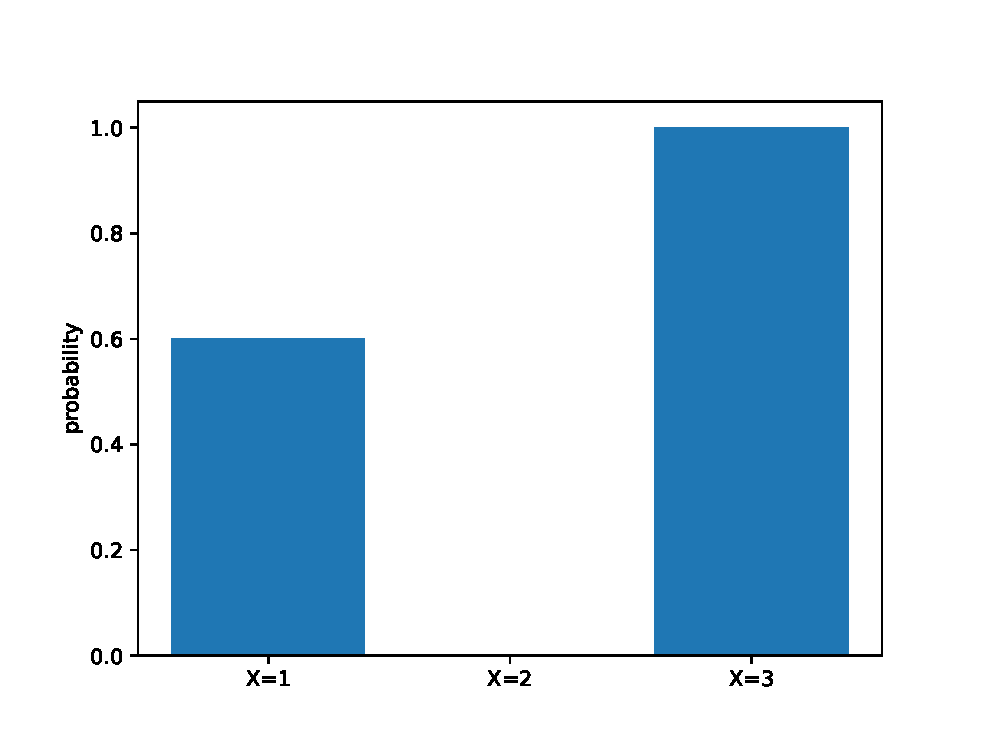
\includegraphics[width=\columnwidth]{./figures/probexm/probexm10.eps}
%	\caption{probability of germinated seeds in a bag }
%	\label{fig:bt10}
%	\begin{lstlisting}
%	figs/probexm/probexm10.eps
%	\end{lstlisting}
%\end{figure}
\end{enumerate}

    \item 1500 families with 2 children were selected randomly, and the following data in Table \ref{table:1.2.2} were recorded.
Compute the probability of a family, chosen at random, having
\begin{enumerate}
\item 2 girls
\item  1 girl
\item  No girl
\end{enumerate}
Also check whether the sum of these probabilities is 1.
\begin{table}[!ht]
\centering
\begin{tabular}{ |c|c|c|c| } 
 \hline
 \textbf{No.of girls in a family} &2 &1 &0\\ 
 \hline
 \textbf{No. of families}  &475 &814 &211\\ 
 \hline 
\end{tabular}
\caption{}
\label{table:1.2.2}
\end{table}
\\
\solution
Let X be the random variable representing the number of defective eggs from the ten eggs picked. X follows a  binomial distribution.  Since the probability of an egg being defective is 10\%, substituting n=10, p= 0.1 and k=0 in equation \eqref{eq:exam41_1}, 
probability that there is atleast one defective egg is 
\begin{align}
\pr{X \geq 1}&= 1 - \pr{X=0}  = 1-\brak{0.9}^{10}
\\
&=0.6513215599
\end{align}
The python code for the above problem is,
\begin{lstlisting}
.solutions/20-10/prob/codes/exam42.py
\end{lstlisting}


\item In a particular section of Class IX, 40 students were asked about the months of their birth and the following graph in Fig. \ref{fig:1.2.3}
was prepared for the data so obtained.     Find the probability that a student of the class was born in August.

\renewcommand{\theequation}{\theenumi}
\begin{enumerate}[label=\arabic*.,ref=\thesubsection.\theenumi]
\numberwithin{equation}{enumi}
\item Eleven bags of wheat flour, each marked 5 kg, actually contained the following weights of flour (in kg):\\
4.97 5.05 5.08 5.03 5.00 5.06 5.08 4.98 5.04 5.07 5.00\\
Find the probability that any of these bags chosen at random contains more than 5 kg of flour.
\end{enumerate}    
\solution
Let X be the random variable representing the number of defective eggs from the ten eggs picked. X follows a  binomial distribution.  Since the probability of an egg being defective is 10\%, substituting n=10, p= 0.1 and k=0 in equation \eqref{eq:exam41_1}, 
probability that there is atleast one defective egg is 
\begin{align}
\pr{X \geq 1}&= 1 - \pr{X=0}  = 1-\brak{0.9}^{10}
\\
&=0.6513215599
\end{align}
The python code for the above problem is,
\begin{lstlisting}
.solutions/20-10/prob/codes/exam42.py
\end{lstlisting}


\item Three coins are tossed simultaneously 200 times with the following frequencies of different outcomeslisted in Table \ref{table:1.2.4}.
If the three coins are simultaneously tossed again, compute the probability of 2 heads coming up.
%
\begin{table}[!ht]
%\resizebox{\columnwidth}{20pt}{%
\resizebox{\columnwidth}{!}{%
\begin{tabular}{ |c|c|c|c|c| } 
 \hline
 \textbf{Outcome} &3 heads &2 heads &1 head &No head\\ 
 \hline
 \textbf{Frequency}  &23 &72 &77 &28\\ 
 \hline
\end{tabular}%\\
}
\caption{}
\label{table:1.2.4}
\end{table}
\\
\solution
Let X be the random variable representing the number of defective eggs from the ten eggs picked. X follows a  binomial distribution.  Since the probability of an egg being defective is 10\%, substituting n=10, p= 0.1 and k=0 in equation \eqref{eq:exam41_1}, 
probability that there is atleast one defective egg is 
\begin{align}
\pr{X \geq 1}&= 1 - \pr{X=0}  = 1-\brak{0.9}^{10}
\\
&=0.6513215599
\end{align}
The python code for the above problem is,
\begin{lstlisting}
.solutions/20-10/prob/codes/exam42.py
\end{lstlisting}

\item Refer to Table \ref{table:1.2.5}.
\begin{enumerate}
\item  Find the probability that a student obtained less than 20$\%$ in the mathematics test.
\item  Find the probability that a student obtained marks 60 or above.
\end{enumerate}
\begin{table}[!ht]
\centering
\begin{tabular}{ |c|c| } 
 \hline
 \textbf{Marks} &\textbf{Number of students}\\
 \hline
  0-20 &7\\ 
  20-30 &10\\ 
  30-40 &10\\ 
  40-50 &20\\ 
  50-60 &20\\ 
  60-70 &15\\ 
  70-above &8\\ 
  \hline
 \textbf{Total}  &90\\ 
 \hline
\end{tabular}
\caption{}
\label{table:1.2.5}
\end{table}
\solution
Let X be the random variable representing the number of defective eggs from the ten eggs picked. X follows a  binomial distribution.  Since the probability of an egg being defective is 10\%, substituting n=10, p= 0.1 and k=0 in equation \eqref{eq:exam41_1}, 
probability that there is atleast one defective egg is 
\begin{align}
\pr{X \geq 1}&= 1 - \pr{X=0}  = 1-\brak{0.9}^{10}
\\
&=0.6513215599
\end{align}
The python code for the above problem is,
\begin{lstlisting}
.solutions/20-10/prob/codes/exam42.py
\end{lstlisting}

\item The distance (in kms) of 40 engineers from their residence to their place of work were found as follows in Table \ref{table:1.2.7}.
What is the empirical probability that an engineer lives
\begin{enumerate}
\item less than 7 km from her place of work?
\item more than or equal to 7 km from her place of work? 
\item within $\frac{1}{2}$km from her place of work?
\end{enumerate}

\begin{table}[!ht]
\centering
\begin{tabular}{ cccccccccc} 

 5 &3 &10 &20 &25 &11 &13 &7 &12 &31\\
 19 &10 &12 &17 &18 &11 &32 &17 &16 &2\\
 7 &9 &7 &8 &3 &5 &12 &15 &18 &3 \\
 12 &14 &2 &9 &6 &15 &15 &7 &6 &12\\ 
 \end{tabular}\\
\caption{}
\label{table:1.2.7}
\end{table}
\solution
Let X be the random variable representing the number of defective eggs from the ten eggs picked. X follows a  binomial distribution.  Since the probability of an egg being defective is 10\%, substituting n=10, p= 0.1 and k=0 in equation \eqref{eq:exam41_1}, 
probability that there is atleast one defective egg is 
\begin{align}
\pr{X \geq 1}&= 1 - \pr{X=0}  = 1-\brak{0.9}^{10}
\\
&=0.6513215599
\end{align}
The python code for the above problem is,
\begin{lstlisting}
.solutions/20-10/prob/codes/exam42.py
\end{lstlisting}



\item An organisation selected 2400 families at random and surveyed them to determine a relationship between income level and the number of vehicles in a family. The information gathered is listed in the Table \ref{table:1.2.8}
Suppose a family is chosen. Find the probability that the family chosen is
\begin{enumerate}
\item  earning \rupee 10000 – \rupee 13000 per month and owning exactly 2 vehicles.
\item  earning \rupee 16000 or more per month and owning exactly 1 vehicle.
\item  earning less than \rupee 7000 per month and does not own any vehicle.
\item  earning \rupee 13000 – \rupee 16000 per month and owning more than 2 vehicles.
\item owning not more than 1 vehicle.
\end{enumerate}
%
\begin{table}[!ht]
\centering
\begin{tabular}{|c|c|c|c|c|}
\hline
\textbf{Monthly income} &\multicolumn{4}{c|}{\textbf{vehicles per family }}\\
\cline{2-5}
(in \textbf{\rupee}) &\textbf{0} &\textbf{1} &\textbf{2} &\textbf{Above 2}\\
\hline
Less than 7000 &10 &160 &25 &0\\
\hline
7000-10000 &0 &305 &27 &2\\
\hline
10000-13000 &1 &535 &29 &1\\
\hline
13000-16000 &2 &469 &59 &25\\
\hline
16000 or more  &1 &579 &82 &88 \\
\hline
\end{tabular}
\caption{}
\label{table:1.2.8}
\end{table}
\solution
Let X be the random variable representing the number of defective eggs from the ten eggs picked. X follows a  binomial distribution.  Since the probability of an egg being defective is 10\%, substituting n=10, p= 0.1 and k=0 in equation \eqref{eq:exam41_1}, 
probability that there is atleast one defective egg is 
\begin{align}
\pr{X \geq 1}&= 1 - \pr{X=0}  = 1-\brak{0.9}^{10}
\\
&=0.6513215599
\end{align}
The python code for the above problem is,
\begin{lstlisting}
.solutions/20-10/prob/codes/exam42.py
\end{lstlisting}


\item Eleven bags of wheat flour, each marked 5 kg, actually contained the following weights of flour (in kg)\\
4.97 5.05 5.08 5.03 5.00 5.06 5.08 4.98 5.04 5.07 5.00\\
Find the probability that any of these bags chosen at random contains more than 5 kg of flour.\\
\solution
%Let X be the random variable representing the number of defective eggs from the ten eggs picked. X follows a  binomial distribution.  Since the probability of an egg being defective is 10\%, substituting n=10, p= 0.1 and k=0 in equation \eqref{eq:exam41_1}, 
probability that there is atleast one defective egg is 
\begin{align}
\pr{X \geq 1}&= 1 - \pr{X=0}  = 1-\brak{0.9}^{10}
\\
&=0.6513215599
\end{align}
The python code for the above problem is,
\begin{lstlisting}
.solutions/20-10/prob/codes/exam42.py
\end{lstlisting}


\item From Table \ref{table:1.2.10}, 
prepare a frequency distribution table, regarding the concentration of sulphur dioxide in the air in parts per million of a certain city for 30 days.   Using this table, find the probability of the concentration of sulphur dioxide in the interval 0.12 - 0.16 on any of these days.
%
\begin{table}[!ht]
\centering
\begin{tabular}{ cccccc} 

  0.03 &0.08 &0.08 &0.09 &0.04 &0.17 \\
 0.16 &0.05 &0.02 &0.06 &0.18 &0.20 \\
 0.11 &0.08 &0.12 &0.13 &0.22 &0.07  \\
 0.08 &0.01 &0.10 &0.06 &0.09 &0.18 \\ 
  0.11 &0.07 &0.05 &0.07 &0.01 &10.04 \\ 
 \end{tabular}\\
\caption{}
\label{table:1.2.10}
\end{table}
\solution
Let X be the random variable representing the number of defective eggs from the ten eggs picked. X follows a  binomial distribution.  Since the probability of an egg being defective is 10\%, substituting n=10, p= 0.1 and k=0 in equation \eqref{eq:exam41_1}, 
probability that there is atleast one defective egg is 
\begin{align}
\pr{X \geq 1}&= 1 - \pr{X=0}  = 1-\brak{0.9}^{10}
\\
&=0.6513215599
\end{align}
The python code for the above problem is,
\begin{lstlisting}
.solutions/20-10/prob/codes/exam42.py
\end{lstlisting}

\item  
A, B, O, O, AB, O, A, O, B, A, O, B, A, O,\\ O,
A, AB, O, A, A, O, O, AB, B, A, O, B, A, B, O.\\
prepare a frequency distribution table regarding the blood groups of 30 students of a class. Use this table to determine the probability that a student of this class, selected at random, has blood group AB.\\
\item Determine P(E/F), if mother, father and son line up at random for a family picture\\
E : son on one end, F : father in middle\\
\item Consider the experiment of throwing a die, if a multiple of 3 comes up, throw the die again and if any other number comes, toss a coin. Find the conditional probability of the event 'the coin shows a tail', given that 'at least one die shows a 3'.\\
\solution
Let $X_k \in \cbrak{-1,0,3,6,r}, k = 1,2, \dots$ represent the described process, where $r,3,6$ denote the outcome of the die and -1,0 denote the outcome of the coin, 0 representing a tail.  In general, the transition probabilities for the Markov Chain are
\begin{align}
\pr{X_n = 0|X_{n-1} = r} &=\pr{X_n = -1|X_{n-1} = r} 
\\
&= \frac{1}{2}
\\
\pr{X_n = 0|X_{n-1} = 3} &=\pr{X_n = -1|X_{n-1} = 3} 
\\
&=0
\\
\pr{X_n = 0|X_{n-1} = 6} &=\pr{X_n = -1|X_{n-1} = 6} 
\\
&=0
\\
\pr{X_n = 3|X_{n-1} = r} &= 0
\\
\pr{X_n = 6|X_{n-1} = r} &= 0
\\
\pr{X_n = r|X_{n-1} = r} &= 0
\\
\pr{X_n = 3|X_{n-1} = 6} &= 
\pr{X_n = 6|X_{n-1} = 3} 
\\
\pr{X_n = 3|X_{n-1} = 3} &= 
\pr{X_n = 6|X_{n-1} = 6} 
\\
&= \frac{1}{6}
\\
\pr{X_n = r|X_{n-1} = 3} &= 
\pr{X_n = r|X_{n-1} = 6} 
\\
= \frac{4}{6}
\end{align}
Thus,
\begin{align}
\pr{X_2 = 0|X_1 = 3} = 0
\end{align}

\item One card is drawn from a well-shuffled deck of 52 cards. Find the probability of getting
(i) a king of red colour\\
(ii) a face card\\
(iii) a red face card\\
(iv) the jack of hearts \\
(v) a spade \\
(vi) the queen of diamonds
\\
\solution
Let X be the random variable representing the number of defective eggs from the ten eggs picked. X follows a  binomial distribution.  Since the probability of an egg being defective is 10\%, substituting n=10, p= 0.1 and k=0 in equation \eqref{eq:exam41_1}, 
probability that there is atleast one defective egg is 
\begin{align}
\pr{X \geq 1}&= 1 - \pr{X=0}  = 1-\brak{0.9}^{10}
\\
&=0.6513215599
\end{align}
The python code for the above problem is,
\begin{lstlisting}
.solutions/20-10/prob/codes/exam42.py
\end{lstlisting}

\item Five cards—the ten, jack, queen, king and ace of diamonds, are well-shuffled with their
face downwards. One card is then picked up at random.\\
(i) What is the probability that the card is the queen?\\
(ii) If the queen is drawn and put aside, what is the probability that the second card
picked up is (a) an ace? (b) a queen?
\\
\solution
Let X be the random variable representing the number of defective eggs from the ten eggs picked. X follows a  binomial distribution.  Since the probability of an egg being defective is 10\%, substituting n=10, p= 0.1 and k=0 in equation \eqref{eq:exam41_1}, 
probability that there is atleast one defective egg is 
\begin{align}
\pr{X \geq 1}&= 1 - \pr{X=0}  = 1-\brak{0.9}^{10}
\\
&=0.6513215599
\end{align}
The python code for the above problem is,
\begin{lstlisting}
.solutions/20-10/prob/codes/exam42.py
\end{lstlisting}

\item A box contains 90 discs which are numbered from 1 to 90. If one disc is drawn at random
from the box, find the probability that it bears (i) a two-digit number (ii) a perfect
square number (iii) a number divisible by 5.
\\
\solution
Let X be the random variable representing the number of defective eggs from the ten eggs picked. X follows a  binomial distribution.  Since the probability of an egg being defective is 10\%, substituting n=10, p= 0.1 and k=0 in equation \eqref{eq:exam41_1}, 
probability that there is atleast one defective egg is 
\begin{align}
\pr{X \geq 1}&= 1 - \pr{X=0}  = 1-\brak{0.9}^{10}
\\
&=0.6513215599
\end{align}
The python code for the above problem is,
\begin{lstlisting}
.solutions/20-10/prob/codes/exam42.py
\end{lstlisting}

\item A child has a die whose six faces show the letters as given in Fig. \ref{fig:130_dice}	.

\begin{figure}[!ht]
\centering
\resizebox{\columnwidth}{!}{%A child has a die whose six faces show the letters as given below:\\

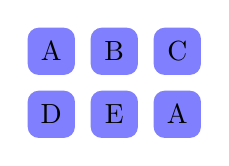
\begin{tikzpicture}[outer sep=0.05cm,node distance=0.8cm,]
\tikzstyle{bigbox} = [draw=white!50, thick, fill=white!10, rounded corners, rectangle]
\tikzstyle{box} = [minimum size=0.6cm, rounded corners,rectangle, fill=blue!50]
%
\node[box] (11) {A};
\node[box,right of=11] (12) {B};
\node[box,right of=12] (13) {C};
\node[box,below of=11] (21) {D};
\node[box,right of=21] (22) {E};
\node[box,right of=22] (23) {A};
\end{tikzpicture}
%\\
%The die is thrown once. What is the probability of getting (i) A? (ii) D?
}
%\resizebox{\columnwidth}{!}{

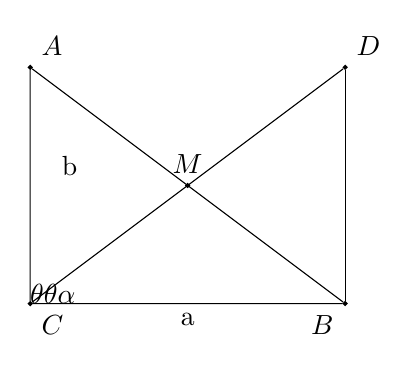
\begin{tikzpicture}
[scale=1,>=stealth,point/.style={draw,circle,fill = black,inner sep=0.5pt},]

%Triangle sides
\def\a{4}
\def\b{3}
\def\c{sqrt(\a^2+\c^2)}



%Labeling points
\node (A) at (0,\b)[point,label=above right:$A$] {};
\node (B) at (\a, 0)[point,label=below left:$B$] {};
\node (C) at (0, 0)[point,label=below right:$C$] {};
\node (M) at (\a*0.5,\b*0.5)[point,label=above:$M$] {};
\node (D) at (\a,\b)[point,label=above right:$D$] {};


%Drawing triangle ABC
\draw (A) -- node[left] {$\textrm{}$} (B) -- node[below] {$\textrm{a}$} (C) -- node[above,xshift=5mm] {$\textrm{b}$} (A);

%Joining CD
\draw (C)--(D);
%Joining BD
\draw (B)--(D);

%Drawing and marking angles
\tkzMarkAngle[fill=orange!40,size=0.5cm,mark=](A,M,C)
\tkzMarkAngle[fill=orange!40,size=0.5cm,mark=](B,M,D)
\tkzMarkAngle[fill=green!40,size=0.5cm,mark=](A,B,C)
\tkzMarkRightAngle[fill=blue!20,size=.2](A,C,B)
\tkzMarkRightAngle[fill=blue!20,size=.2](D,B,C)
\tkzLabelAngle[pos=0.65](A,M,C){$\theta$}
\tkzLabelAngle[pos=0.65](B,M,D){$\theta$}
\tkzLabelAngle[pos=0.65](A,B,C){$\alpha$}


\end{tikzpicture}
}
\caption{}
\label{fig:130_dice}	
\end{figure}

The die is thrown once. What is the probability of getting (i) A? (ii) D?
\\
\solution
Let X be the random variable representing the number of defective eggs from the ten eggs picked. X follows a  binomial distribution.  Since the probability of an egg being defective is 10\%, substituting n=10, p= 0.1 and k=0 in equation \eqref{eq:exam41_1}, 
probability that there is atleast one defective egg is 
\begin{align}
\pr{X \geq 1}&= 1 - \pr{X=0}  = 1-\brak{0.9}^{10}
\\
&=0.6513215599
\end{align}
The python code for the above problem is,
\begin{lstlisting}
.solutions/20-10/prob/codes/exam42.py
\end{lstlisting}

\item Which of the following arguments are correct and which are not correct? Give reasons
for your answer.\\
(i) If two coins are tossed simultaneously there are three possible outcomes—two
heads, two tails or one of each. Therefore, for each of these outcomes, the
probability is $\frac{1}{3}$ \\
(ii) If a die is thrown, there are two possible outcomes—an odd number or an even
number. Therefore, the probability of getting an odd number is $\frac{1}{2}$.
\\
\solution
\renewcommand{\theequation}{\theenumi}
\begin{enumerate}[label=\arabic*.,ref=\thesubsubsection.\theenumi]
\numberwithin{equation}{enumi}
\item In the given question,
\\
The sample size = Total number of possibilities(S)=6
\begin{align}
\myvec{1&2&3&4&5&6}
\end{align}
Event size= Odd number =3
\begin{align}
\myvec{1&3&5}
\end{align}
Probability for this event is = $\frac{1}{2}$
\\
The python code for the distribution of data,
\begin{lstlisting}
prob/codes/prob6_b.py
\end{lstlisting}
This shows the diagrametic representation of dice with the live update of probability with the role of dice.
\end{enumerate}

\item Two customers Shyam and Ekta are visiting a particular shop in the same week (Tuesday
to Saturday). Each is equally likely to visit the shop on any day as on another day. What
is the probability that both will visit the shop on\\
(i) the same day?\\
(ii) consecutive days?\\
(iii) different days?
\\
\solution
Let X be the random variable representing the number of defective eggs from the ten eggs picked. X follows a  binomial distribution.  Since the probability of an egg being defective is 10\%, substituting n=10, p= 0.1 and k=0 in equation \eqref{eq:exam41_1}, 
probability that there is atleast one defective egg is 
\begin{align}
\pr{X \geq 1}&= 1 - \pr{X=0}  = 1-\brak{0.9}^{10}
\\
&=0.6513215599
\end{align}
The python code for the above problem is,
\begin{lstlisting}
.solutions/20-10/prob/codes/exam42.py
\end{lstlisting}

\item A die is numbered in such a way that its faces show the numbers 1, 2, 2, 3, 3, 6. It is thrown two times and the total score in two throws is noted. Complete the following
table which gives a few values of the total score on the two throws:
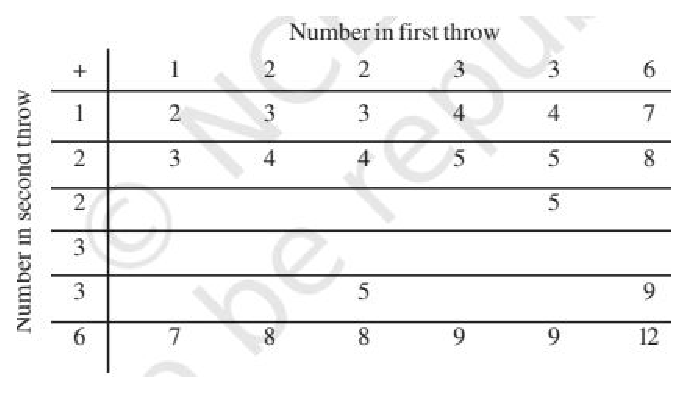
\includegraphics[width=\columnwidth]{./prob/figs/rows.eps}\\
What is the probability that the total score is
(i) even? (ii) 6? (iii) at least 6?
\\
\solution
Let X be the random variable representing the number of defective eggs from the ten eggs picked. X follows a  binomial distribution.  Since the probability of an egg being defective is 10\%, substituting n=10, p= 0.1 and k=0 in equation \eqref{eq:exam41_1}, 
probability that there is atleast one defective egg is 
\begin{align}
\pr{X \geq 1}&= 1 - \pr{X=0}  = 1-\brak{0.9}^{10}
\\
&=0.6513215599
\end{align}
The python code for the above problem is,
\begin{lstlisting}
.solutions/20-10/prob/codes/exam42.py
\end{lstlisting}


\end{enumerate}

